%%%%%%%%%%%%%%%%%%%%%%%%%%%%%%%%%%%%%%%%%%%%%%%%%%%%%%%%%%%%%%%%%%%%%%%%

%%% The code below was generated by the tool at http://dl.acm.org/ccs.cfm.
%%% Please replace this example with code appropriate for your own paper.

%%%%%%%%%%%%%%%%%%%%%%%%%%%%%%%%%%%%%%%%%%%%%%%%%%%%%%%%%%%%%%%%%%%%%%%%

%%% LaTeX Template for AAMAS-2025 (based on sample-sigconf.tex)
%%% Prepared by the AAMAS-2025 Program Chairs based on the version from AAMAS-2025. 

%%%%%%%%%%%%%%%%%%%%%%%%%%%%%%%%%%%%%%%%%%%%%%%%%%%%%%%%%%%%%%%%%%%%%%%%

%%% Start your document with the \documentclass command.


%%% == IMPORTANT ==
%%% Use the first variant below for the final paper (including auithor information).
%%% Use the second variant below to anonymize your submission (no authoir information shown).
%%% For further information on anonymity and double-blind reviewing, 
%%% please consult the call for paper information
%%% https://aamas2025.org/index.php/conference/calls/submission-instructions-main-technical-track/

%%%% For anonymized submission, use this
\documentclass[sigconf,anonymous]{aamas} 
\begin{CCSXML}
<ccs2012>
    <concept>
        <concept_id>10010147.10010178.10010199.10010202</concept_id>
        <concept_desc>Computing methodologies~Multi-agent planning</concept_desc>
        <concept_significance>500</concept_significance>
        </concept>
  </ccs2012>
\end{CCSXML}
\ccsdesc[500]{Computing methodologies~Multi-agent planning}
%%%% For camera-ready, use this
% \documentclass[sigconf]{aamas} 

%%% Load required packages here (note that many are included already).

\usepackage{balance} % for balancing columns on the final page
% new package
\usepackage{algorithm}
% \usepackage{algorithmic}
\usepackage{algpseudocode}
\usepackage{amsmath}
% \usepackage[linesnumbered,ruled,vlined]{algorithm2e}
\usepackage{graphicx}
\usepackage{subfigure}
\usepackage{url}
\renewcommand{\algorithmicrequire}{\textbf{Input:}}
\renewcommand{\algorithmicensure}{\textbf{Output:}}
%%%%%%%%%%%%%%%%%%%%%%%%%%%%%%%%%%%%%%%%%%%%%%%%%%%%%%%%%%%%%%%%%%%%%%%%

%%% AAMAS-2025 copyright block (do not change!)

\setcopyright{ifaamas}
\acmConference[AAMAS '25]{Proc.\@ of the 24th International Conference
on Autonomous Agents and Multiagent Systems (AAMAS 2025)}{May 19 -- 23, 2025}
{Detroit, Michigan, USA}{A.~El~Fallah~Seghrouchni, Y.~Vorobeychik, S.~Das, A.~Nowe (eds.)}
\copyrightyear{2025}
\acmYear{2025}
\acmDOI{}
\acmPrice{}
\acmISBN{}


%%%%%%%%%%%%%%%%%%%%%%%%%%%%%%%%%%%%%%%%%%%%%%%%%%%%%%%%%%%%%%%%%%%%%%%%

%%% == IMPORTANT ==
%%% Use this command to specify your EasyChair submission number.
%%% In anonymous mode, it will be printed on the first page.

\acmSubmissionID{<<EasyChair submission id>>}

%%% Use this command to specify the title of your paper.

\title[AAMAS-2025 Formatting Instructions]{Task Group Allocation for Solving Multi-Load Agent Pickup and Delivery problem}

%%% Provide names, affiliations, and email addresses for all authors.

\author{Hao Ye}
\affiliation{
  \institution{Harbin Institute of Technology (Shenzhen)}
  \city{Shenzhen}
  \country{China}}
\email{yehao@stu.hit.edu.cn}

\author{Yifei Li}
\affiliation{
  \institution{Harbin Institute of Technology (Shenzhen)}
  \city{Shenzhen}
  \country{China}}
\email{liyifei@stu.hit.edu.cn}

\author{Hejiao Huang}
\affiliation{
  \institution{Harbin Institute of Technology (Shenzhen)}
  \city{Shenzhen}
  \country{China}}
\email{huanghejiao@hit.edu.cn}

%%% Use this environment to specify a short abstract for your paper.

\begin{abstract}
This document outlines the formatting instructions for submissions to
AAMAS-2025. You can use its source file as a template when writing 
your own paper. It is based on the file `\texttt{sample-sigconf.tex}'
distributed with the ACM article template for \LaTeX\@.
\end{abstract}

%%% The code below was generated by the tool at http://dl.acm.org/ccs.cfm.
%%% Please replace this example with code appropriate for your own paper.


%%% Use this command to specify a few keywords describing your work.
%%% Keywords should be separated by commas.

\keywords{Multi-load agent, Pickup and delivery problem, Task allocation}

%%%%%%%%%%%%%%%%%%%%%%%%%%%%%%%%%%%%%%%%%%%%%%%%%%%%%%%%%%%%%%%%%%%%%%%%

%%% Include any author-defined commands here.
         
\newcommand{\BibTeX}{\rm B\kern-.05em{\sc i\kern-.025em b}\kern-.08em\TeX}

%%%%%%%%%%%%%%%%%%%%%%%%%%%%%%%%%%%%%%%%%%%%%%%%%%%%%%%%%%%%%%%%%%%%%%%%

\begin{document}

%%% The following commands remove the headers in your paper. For final 
%%% papers, these will be inserted during the pagination process.

\pagestyle{fancy}
\fancyhead{}

%%% The next command prints the information defined in the preamble.

\maketitle 

\section{Introduction}
The multi-load agent pickup and delivery problem (MLAPD) is a variant of the pickup and delivery problem
which is a well-known combinatorial optimization problem in the field of logistics and transportation.
In the MLAPD problem, there are multiple agents, each of which can carry multiple tasks at the same time.
The goal is to allocate tasks to agents to optimize the completion time of all tasks.
The MLAPD problem is a NP-hard problem, and it is difficult to solve it optimally in polynomial time~\cite{bai2022group}.

\section{Related Work}
\section{PROBLEM DEFINITION}
In this section, we introduce the multi-load agent pickup and delivery problem, 
which we address in this paper. 
Before this, we first give the definitions of map, task, agent, comparative metrics and MLAPD problem.

\begin{definition}[Map]
\label{MapDfn}
    A map $G = (V, E)$ is the , 
    whose vertices $V$ correspond to locations and edges $E$ represent edges between adjoining locations.
    The shortest distance of the path between two locations $v_{i}$ and $v_{j}$ is denoted as $dis(v_{i}, v_{j})$.

\end{definition}

\begin{definition}[Task]
\label{TaskDfn}
    A task $\tau \in \Gamma$ is a tuple 
    $<v^{s}_{\tau}, v^{g}_{\tau}, t^{r}_{\tau}, t^{d}_{\tau}, t^{c}_{\tau}>$, 
    where $v^{s}_{\tau}$ and $v^{g}_{\tau}$ are the pickup location and delivery location, respectively. 
    $t^{r}_{\tau}, t^{d}_{\tau}$ and $t^{c}_{\tau}$ are the release time, deadline and completed time, respectively.
\end{definition}

% Task Group ?

\begin{definition}[Agent]
\label{AgentDfn}
    An agent $a \in A$ is represented as a tuple $<v_{a}, c_{a}, \Gamma_{a}, S_{\Gamma_{a}}>$, 
    where $v_{a}$ is location, $c_{a}$ represents the maximum capacity, 
    $\Gamma_{a}$ is the set of tasks, and $S_{\Gamma_{a}}$ is the schedule of $\Gamma_{a}$. 
    The $S_{\Gamma_{a}} = <v_{1}, v_{2},..., v_{n}>$, 
    where $v_{i}$ is a pickup or delivery location of task $\tau \in \Gamma_{a}$,
    and the cost of schedule $S_{\Gamma_{a}}$ is denoted as 
    $Cost(S_{\Gamma_{a}}) = \sum^{n-1}_{i=1}{dis(v_i, v_{i+1})}$.
\end{definition}

A task $\tau \in \Gamma$ is released at $t^{r}_{\tau}$. 
When system assigns $\tau$ to an agent $a$, 
$a$ needs to reach $v^{s}_{\tau}$ before $t^{d}_{\tau}$, 
and then deliver $\tau$ to $v^g_{\tau}$ while recording the completed time $t^{c}_{\tau}$. 
If $\tau$ could not be completed before $t^{d}_{\tau}$, 
then the task is considered as failed.

\begin{definition}[Comparative metrics]
    In this paper, we demonstrate algorithmic superiority through three comparative metrics, 
    service time (${ST}$), makespan ($MS$) and completion ratio ($CR$). 
    $ST = \sum_{\tau_i \in \Gamma}{(t^{c}_{\tau_i} - t^{r}_{\tau_i})}$, 
    is defined as the sum of differences between the completed times and the release times of all tasks.
    $MS = max{\{t^{c}_{\tau}\}}$ $(\forall \tau \in \Gamma)$ 
    is time when last task has completed.
    $CR = {\sum_{\tau_i \in \Gamma}{X_{\tau_i}}}/{|\Gamma|}$, 
    where $X_{\tau_i}$ is a decision variable, is completion ratio of $\Gamma$. 
    If task $\tau_{i}$ is completed, then $X_{\tau_i}$ is 1; otherwise, it is 0.
       
\end{definition}

\begin{definition}[MLAPD]
\label{ProDfn}
    The multi-load agent pickup and delivery problem (MLAPD) is a tuple $P = <G, A, \Gamma>$, 
    defined by a map $G$, a set of agents $A$, and a set of tasks $\Gamma$. 
    Moreover, $P$ amounts to finding the allocation of tasks to agents, 
    which optimize three comparative indicators, ($ST, MS, CR$).
    Time is discretized into timesteps, and agents can only move to adjacent locations 
    or wait at its current location in one timestep.
    Howerver, a conflict occurs when two agents are at the same location or pass through the same edge at the same time.
    The time required to avoid conflicts needs to be considered, since it will affect the comparative metrics.
    Therefore, we assue that agents can take $\theta$ time to avoid a conflict.
\end{definition}
 
\section{Solution}

In this study, Task-Group Allocation Algorithm (TGA) is developed to solve MLAPD problem efficiently. 
The TGA method first analyzes the likelihood of carpooling between each task, 
and then divide the set of tasks into groups via K-Capacity Hierarchical Clustering Algorithm (KCHC). 
Then, we allocate task groups to agents.

\subsection{Carpooling Chance}
% 说明为什么搞task group
The biggest difference between multi-load agent and single-load agent 
is that multi-load agent can load multiple items at the same time. 
This means that multi-load agent performing a task affects the completion time of the "co-passenger" tasks 
which are also executed to the same agent at same time.
\begin{figure}[ht]
  \centering
  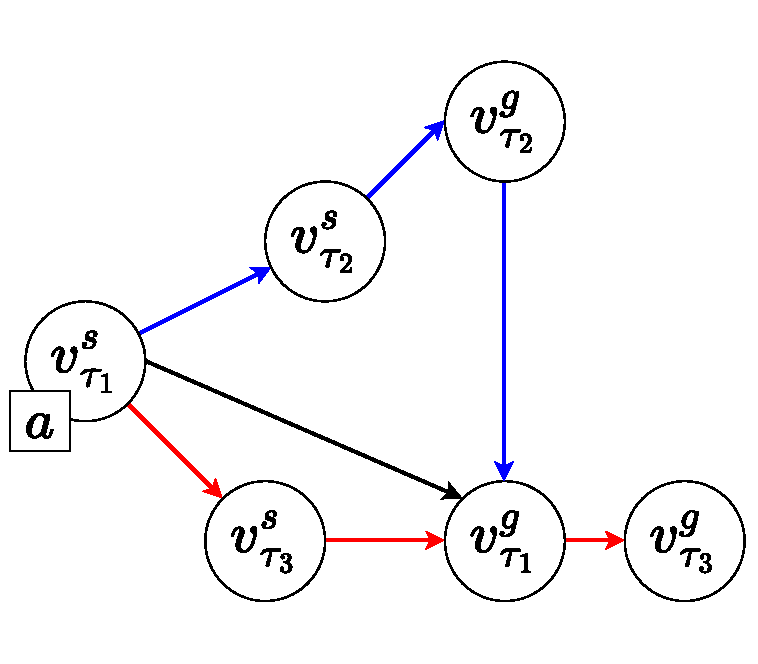
\includegraphics[width=0.5\linewidth]{Fig/carpooling.pdf}
  \caption{The impact of co-passenger tasks}
  \label{fig:carpooling}
  \Description{The impact of co-passenger tasks}
\end{figure}

\begin{example}[Co-passenger tasks]
As shown as in Figure~\ref{fig:carpooling}, there is an agent, $a$, 
and three tasks, $\tau_{1}$, $\tau_{2}$ and $\tau_{3}$.
The agent $a$ is located at pickup location of $\tau_{1}$.
The blue lines are the best schedule for agent $a$ to complete $\tau_{1}$ and $\tau_{2}$.
The red lines are the best schedule for agent $a$ to complete $\tau_{1}$ and $\tau_{3}$.
When we allocate $\tau_{1}$ and $\tau_{2}$ to the agent $a$,
the agent $a$ needs to take the blue paths to complete $\tau_{1}$ and $\tau_{2}$ by greedy strategy,
and it will not impact the completion time of $\tau_{2}$ but lengthen the completed time of $\tau_{1}$.
Howerver, if we allocate $\tau_{1}$ and $\tau_{3}$ to the agent $a$, 
$a$ needs to take the red paths to complete $\tau_{1}$ and $\tau_{3}$.
While it also lengthens the completed time of $\tau_{1}$, 
it is obvious that $\tau_3$ has less of an effect on $\tau_1$ as compared to $\tau_{2}$.
Therefore, we need to consider the impact of "co-passenger" tasks when allocating tasks to agents.
\end{example}


\begin{figure}[htbp]
  \centering
  \subfigure[$S^1_{i,j}$]{
    \label{fig:schedule1}
    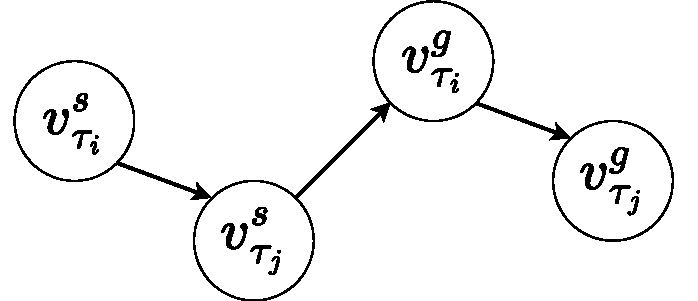
\includegraphics[width=0.4\linewidth]{Fig/path1.pdf}}
  \subfigure[$S^2_{i,j}$]{
    \label{fig:schedule2}
    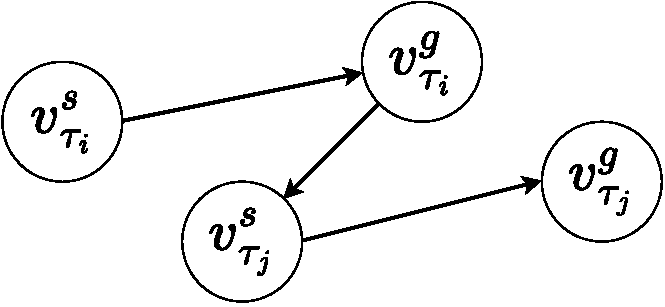
\includegraphics[width=0.4\linewidth]{Fig/path2.pdf}}
  \subfigure[$S^3_{i,j}$]{
    \label{fig:schedule3}
    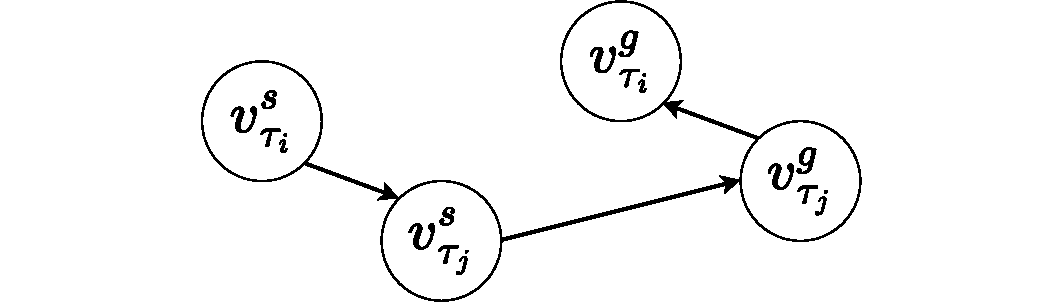
\includegraphics[width=0.4\linewidth]{Fig/path3.pdf}}
  \subfigure[$S^4_{i,j}$]{
    \label{fig:schedule4}
    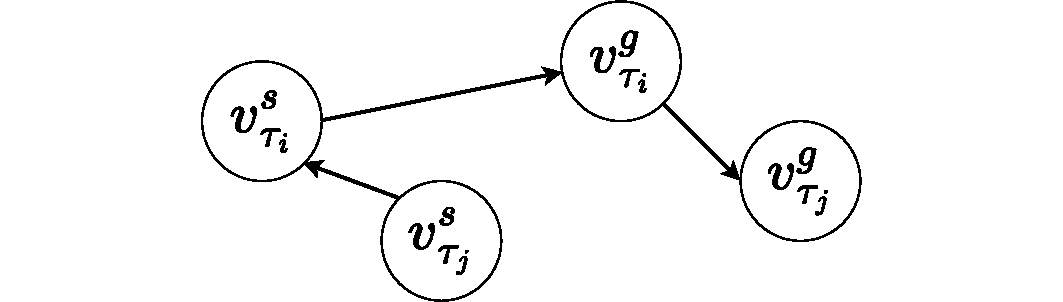
\includegraphics[width=0.4\linewidth]{Fig/path4.pdf}}
  \subfigure[$S^5_{i,j}$]{
    \label{fig:schedule5}
    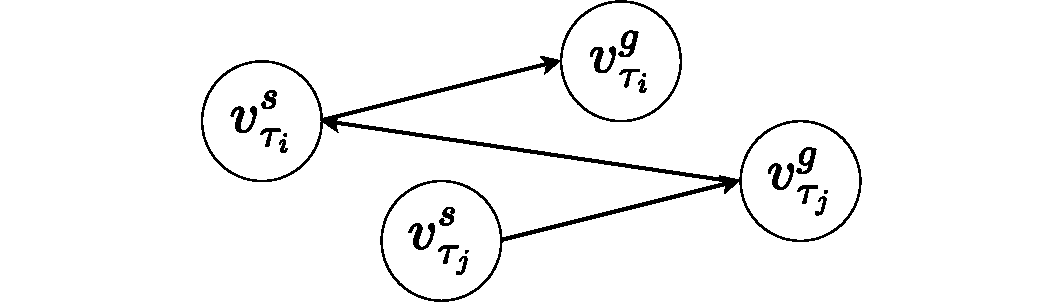
\includegraphics[width=0.4\linewidth]{Fig/path5.pdf}}
  \subfigure[$S^6_{i,j}$]{
    \label{fig:schedule6}
    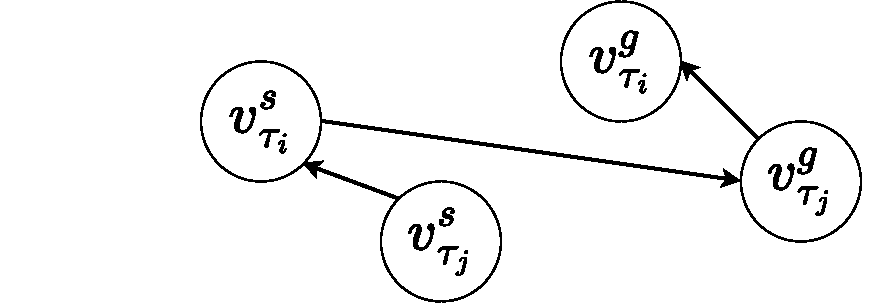
\includegraphics[width=0.4\linewidth]{Fig/path6.pdf}}
  \caption{All possible schedules of two tasks}
  \label{fig:2TP}
  \Description{All possible schedules of two tasks}
\end{figure}

We first analyze the likelihood of carpooling between two tasks.
As shown in Figure~\ref{fig:2TP}, there are 6 schedules to the completion of $\tau_{i}$ and $\tau_{j}$, 
ignoring the location of agent.
The schedules are $S^{1}_{i,j}$, $S^{2}_{i,j}$, $S^{3}_{i,j}$, $S^{4}_{i,j}$, $S^{5}_{i,j}$ and $S^{6}_{i,j}$.
Therefore, we define the carpooling chance between two tasks $\tau_{i}$ and $\tau_{j}$ as follows.

\begin{definition}[Carpooling chance]
\label{cp2}
    The carpooling chance between two tasks $\tau_{i}$ and $\tau_{j}$ is defined as 
    \begin{eqnarray}
    \label{eq:cp2}
        \delta_{\tau_{i}, \tau_{j}} = min\{Cost(S^{q}_{i,j})\} - 
        dis(v^{g}_{\tau_{i}}, v^{s}_{\tau_{i}}) - dis(v^{g}_{\tau_{j}}, v^{s}_{\tau_{j}})
        % q \in \{1, 2, 3, 4, 5, 6\}
    \end{eqnarray}
    where $q \in [1, 6] \wedge q \in \mathbb{N_+}$. $\delta_{i,j}$ is difference 
    between the best schedule of two tasks 
    and the sum of the distances between the pickup and delivery locations of the two tasks.
    The small $\delta_{i,j}$ indicates that $\tau_{i}$ and $\tau_{j}$ being executed by the same agent
    has less impact on each other's completed time, which can efficiently optimize ${ST}$.
\end{definition}

Howerver, in this paper, we focus on multi-load agents, 
which can carry multiple tasks at the same time, not just two agents.
Therefore, we need to consider the carpooling chance between multiple tasks.
In the beginning, we encounter an issue 
that we cannot find the best schedule to complete multiple tasks, 
which is a NP-hard problem.
Therefore, we firtly find a novel schedule to complete there tasks.
Then we evaluate cost of the schedule and proof it.
Finally, we quantify the carpooling chance between multiple tasks.

As shown in Figure~\ref{fig:K-taskgroup}, there is a set of task $\Gamma_K$, 
which contains K tasks, $\tau_{1}$, $\tau_{2}$, ..., $\tau_{K}$.
The schedule $\dot{S_{\Gamma_K}}$ of K tasks is shown in Figure~\ref{fig:KTG-path}.
This schedule starts at the pickup location of a task in $\Gamma_K$, 
then goes to the pickup location of other tasks in $\Gamma_K$, 
and finally to the delivery location of all tasks in $\Gamma_K$.
More significantly, in $\dot{S_{\Gamma_K}}$,
the path between two locations about two tasks in $\Gamma_K$ 
is is part of paths of the best schedules of two tasks.
Therefore, Theorem~\ref{thm:TaskGroupCost} is proposed to evaluate the cost of the schedule of K tasks,
and prove it.

\begin{figure}[ht]
  \centering
  \subfigure[$\Gamma_K$]{
    \label{fig:K-taskgroup}
    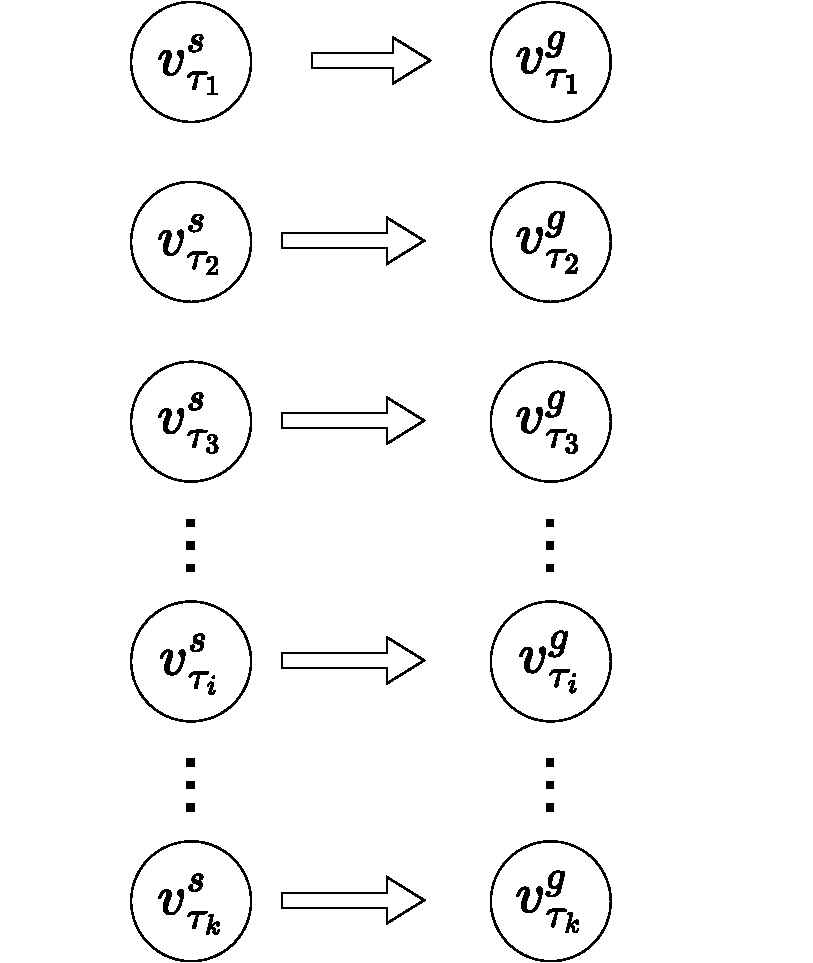
\includegraphics[width=0.4\linewidth]{Fig/k-tasks.pdf}}
  \subfigure[Schedule of $\Gamma_K$]{
    \label{fig:KTG-path}
    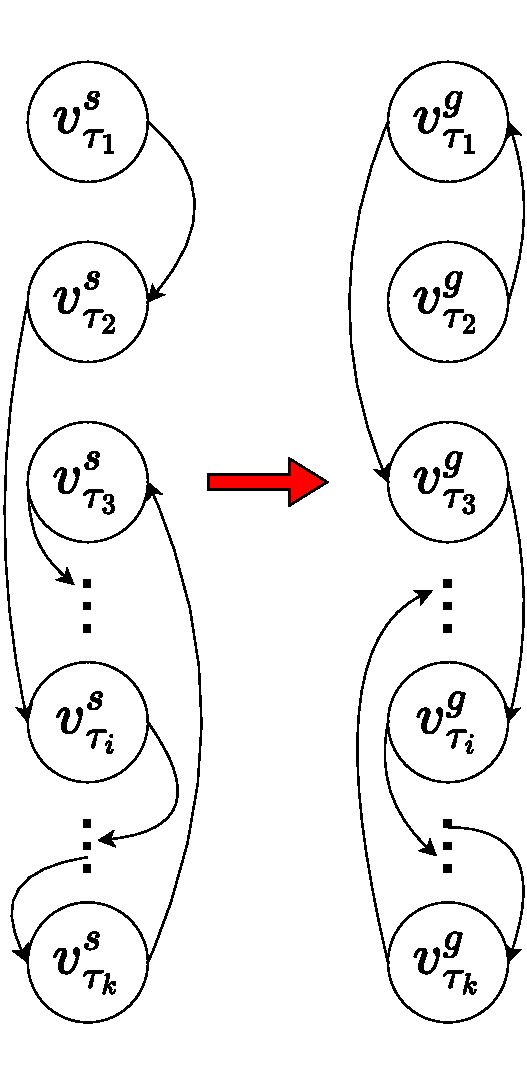
\includegraphics[width=0.4\linewidth]{Fig/Path-KT.pdf}}
  \caption{Schedule of K Tasks}
  \label{PKT}
  \Description{Schedule of K Tasks}
\end{figure}

\begin{theorem}
    \label{thm:TaskGroupCost}
    Given a set of tasks $\Gamma_K$, there exists a path shown in Figure~\ref{fig:KTG-path} 
    such that the following bound holds.
    
    \begin{eqnarray}
        \label{eq:tgc}
        Cost(\dot{S_{\Gamma_K}}) \leq 2 {\ast} \sum_{\tau_i \in \Gamma_K}{dis(v^{s}_{\tau_i}, v^{g}_{\tau_i})} 
        + 2{\ast}(K-1)\delta
    \end{eqnarray}
    where $\delta$ is the carpooling chance between two tasks.
\end{theorem}

\begin{figure}[ht]
  \centering
  \subfigure[Tournament]{
  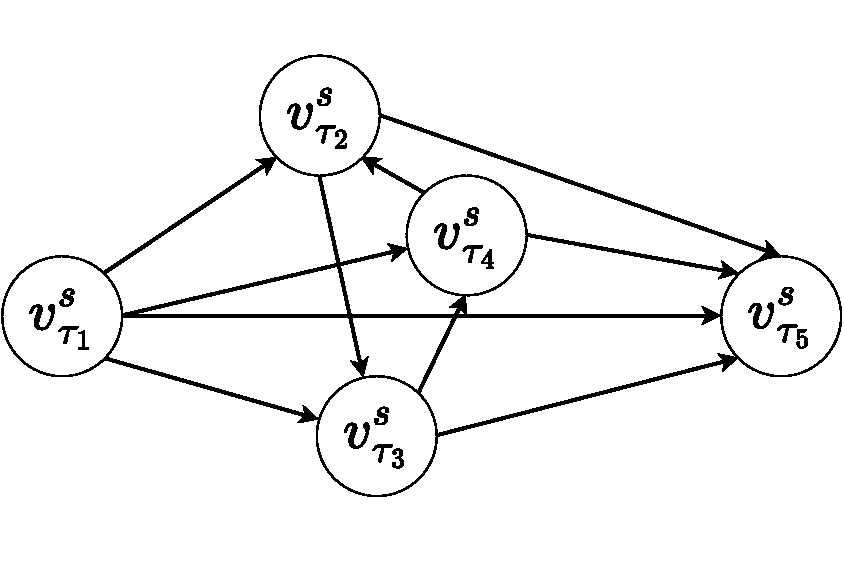
\includegraphics[width=0.3\linewidth]{Fig/tournament.pdf}
  \label{fig:tournament}}
  \subfigure[SCC]{
  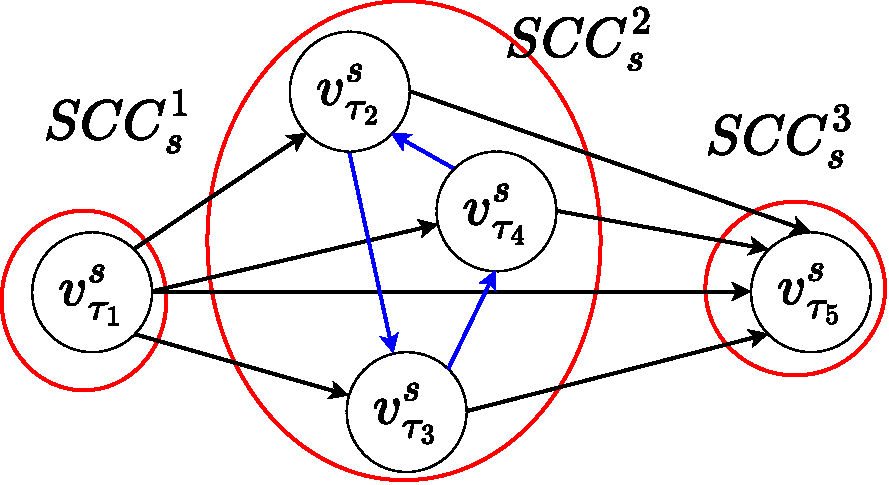
\includegraphics[width=0.3\linewidth]{Fig/SCCs.pdf}
  \label{SCC}}
  % \subfigure[suodian]{
  % 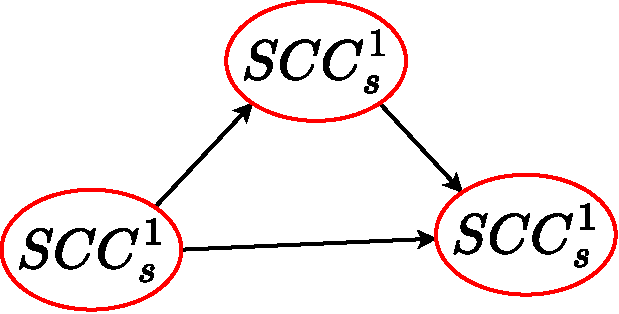
\includegraphics[width=0.4\linewidth]{Fig/suodian.pdf}
  % \label{fig:suodian}}
  \subfigure[topologize]{
  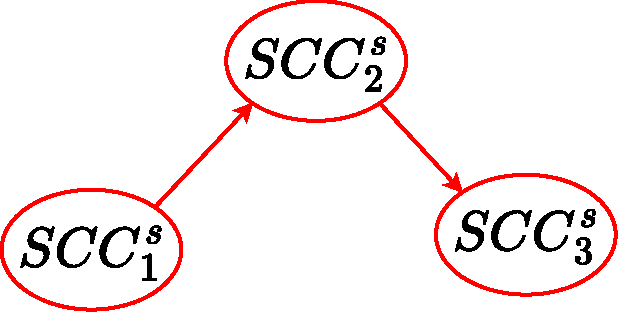
\includegraphics[width=0.3\linewidth]{Fig/topologize.pdf}
  \label{fig:topologize}}
  \caption{The tournament and SCC}
  \label{fig:tournament-SCC}
  \Description{The tournament and SCC}
\end{figure}

\begin{proof}
    Firstly, we need to prove that there is a path to complete $\Gamma_K$.
    As shown in Figure~\ref{fig:KTG-path},
    the schedule first connects the pickup locations of all tasks in $\Gamma_K$,
    then connects the delivery locations of all tasks in $\Gamma_K$.
    Focusing on the pickup locations set of $\Gamma_K$
    and connecting the pickup locations,
    we can get a tournament~\cite{enwiki:1234378036}, 
    which is a directed graph with exactly one edge between each two vertices, 
    in one of the two possible directions.
    As shown in Figure~\ref{fig:tournament}, 
    there are 5 pickup locations,
    and a path between each two locations.
    Accroding to the definition of tournament,
    there is a Hamiltonian path in the tournament~\cite{enwiki:1234378036},
    that means there exists a path to connect all pickup locations of $\Gamma_K$.
    Similarly, there is a path to connect all delivery locations of $\Gamma_K$.
    Then, we need to find a path to connect the pickup locations and delivery locations.
    Therefore, we introduce the Strongly Connected Component (SCC)~\cite{SCC},
    which is a subgraph that is strongly connected.
    As shown in Figure~\ref{SCC},
    $v^{s}_{\tau_{2}}$, $v^{s}_{\tau_{3}}$ and $v^{s}_{\tau_{4}}$ combine  to form a SCC
    where there is a path between each two locations.
    When we shrink the SCC to a single vertex 
    and focus on the last SCC of the pickup locations and first SCC of the delivery locations,
    we can find two locations, $v^{s}_{\tau_{i}}$ and $v^{g}_{\tau_{j}}$, in two SCCs respectively.
    Therefore, there is a path between $v^{s}_{\tau_{i}}$ and $v^{g}_{\tau_{j}}$ 
    to connect the pickup locations and delivery locations.
    % proof that in appendix

    Secondly, we need to evaluate the cost of the path.
    In the beginning, we evaluate the cost of the path between the pickup locations.
    $dis(v^{s}_{\tau_{j}}, v^{s}_{\tau_{i}})$ is the distance 
    between the pickup locations of $\tau_{i}$ and $\tau_{j}$,
    and all possible schedules of two tasks are shown in Figure~\ref{fig:2TP}.
    If the best schedule of two tasks is $S^{1}_{i,j}$,
    we can get Equation~\ref{eq:dis1}.
    \begin{eqnarray}
      \label{eq:dis1}
      Cost(S^{1}_{i,j}) &=& dis(v^s_{\tau_j}, v^s_{\tau_i})+dis(v^g_{\tau_i}, v^s_{\tau_j})
      +dis(v^g_{\tau_j}, v^g_{\tau_i}) \nonumber \\
      % dis(v^g_{\tau_j}, v^s_{\tau_j}) + dis(v^g_{\tau_i}, v^s_{\tau_i}) + \delta_{\tau_i, \tau_j}
      & \geq & dis(v^s_{\tau_j}, v^s_{\tau_i})+ dis(v^g_{\tau_j}, v^s_{\tau_j})\\
      \label{eq:dis2}
      dis(v^g_{\tau_i}, v^s_{\tau_i})+\delta_{\tau_i, \tau_j} &\geq& dis(v^s_{\tau_j}, v^s_{\tau_i})
    \end{eqnarray}
    Then, based on this Definition~\ref{cp2}, we can get Equation~\ref{eq:dis2}.
    Finally, we check all the possible schedules of two tasks in Figure~\ref{fig:2TP},
    and we ensure the Equation~\ref{eq:dis2} holds.
    Similarly, we can evaluate the cost of the path between the delivery locations
    by the same method and get Equation~\ref{eq:dis3}.
    \begin{eqnarray}
      \label{eq:dis3}
      dis(v^{g}_{\tau_{j}}, v^{s}_{\tau_{j}})+ \delta_{i,j} &\geq& dis(v^{g}_{\tau_{j}}, v^{g}_{\tau_{i}})
    \end{eqnarray}
    Therefore, we can evaluate the cost of the path between the pickup locations and delivery locations.
    The cost of paths in pickup locations less than or equal to 
    $\sum_{\tau_i \in {\Gamma_K \setminus \tau_i}}{dis(v^{s}_{\tau_i}, v^{g}_{\tau_i})}$ + $(K-1)\delta$,
    which $\tau_i$ is the last pickup location in $\dot{S_{\Gamma_K}}$.
    The cost of paths in delivery locations less than or equal to
    $\sum_{\tau_i \in \Gamma_K \setminus \tau_j}{dis(v^{s}_{\tau_i}, v^{g}_{\tau_i})}$ + $(K-1)\delta$,
    which $\tau_j$ is the first delivery location in $\dot{S_{\Gamma_K}}$.
    The cost of the path $dis(v^{g}_{\tau_{j}}, v^{s}_{\tau_{i}})$, 
    which connects the pickup locations and delivery locations in $\dot{S_{\Gamma_K}}$,
    is less than or equal to $dis(v^{g}_{\tau_{j}}, v^{s}_{\tau_{j}}) + dis(v^{g}_{\tau_{i}}, v^{s}_{\tau_{i}})$.
    Therefore, the cost of the schedule is less than or equal to 
    $2 {\ast} \sum_{\tau_i \in \Gamma_K}{dis(v^{s}_{\tau_i}, v^{g}_{\tau_i})} + 2{\ast}(K-1)\delta$.

\end{proof}


Therefore, we can quantify the carpooling chance between multiple tasks as follows,
and introduce the Get Carpooling Chance Algorithm (GCC).
Accroding to the Theorem~\ref{thm:TaskGroupCost},
to be more efficient,
we fisrt use Tarjan algorithm~\cite{tarjan1972depth} to get the SCCs of the set of tasks,
and topologize it to get chain of SCC like Figure~\ref{fig:topologize}.
Then, we calculate the carpooling chance in each SCC by Equation~\ref{eq:inSCC},
and between two SCCs by Equation~\ref{eq:betweenSCC}.
Finally, we get the carpooling chance between two task groups by Algorithm~\ref{alg:GCC}.
\begin{eqnarray}
  \label{eq:inSCC}
    \Delta_{SCC} =\frac{2 {\ast} \sum_{\tau_i \in SCC}{\sum_{\tau_j \in SCC}{\delta_{\tau_i, \tau_j}}} }
    {|SCC|}\\
  \label{eq:betweenSCC}
    \Delta_{SCC_i, SCC_{i+1}} = \frac{\sum_{\tau_i \in SCC_i}{\sum_{\tau_j \in SCC_{i+1}}{\delta_{\tau_i, \tau_j}}} }
    {|SCC^i|{\ast}|SCC^{i+1}|}
\end{eqnarray}

\begin{algorithm}[htbp]
\caption{Get Carpooling Chance Algorithm}
\label{alg:GCC}
\begin{algorithmic}[1]
\Require Set of tasks $\Gamma_K$ %%input
\Ensure Carpooling chance $\Delta_{\Gamma_K}$ %%output
\State Initialize $\Delta_{\Gamma_K} = 0$
\State Call Tarjan algorithm to get $SCC^s$ and $SCC^g$ of $\Gamma_K$
\For {$SCC^s_{i} \in SCC^s$}
    \State $\Delta_{SCC^s_i} =\frac{2 {\ast} \sum_{\tau_i \in SCC^s_{i}}{\sum_{\tau_j \in SCC^s_{i}}{\delta_{\tau_i, \tau_j}}} }
    {|SCC^s_{i}|}$
    \If {$SCC^s_i$ is not last SCC}
        \State $\Delta_{SCC^s_i, SCC^s_{i+1}} = \frac{\sum_{\tau_i \in SCC^s_i}{\sum_{\tau_j \in SCC^s_{i+1}}{\delta_{\tau_i, \tau_j}}} }
        {|SCC^s_i|{\ast}|SCC^s_{i+1}|}$
    \EndIf
    \State $\Delta_{\Gamma_K} += \Delta_{SCC}$ + $\Delta_{SCC^s_i, SCC^s_{i+1}}$
\EndFor
\State Do the same for $SCC^g$
\State \Return $\Delta_{\Gamma_K}$
\end{algorithmic}
\end{algorithm}

\textbf{Algorithm Detail:} 
The pseduo-code of Get Carpooling Chance Algorithm is shown in Algorithm~\ref{alg:GCC},
where the input is a set of tasks $\Gamma_K$ containing K tasks,
and the output is the carpooling chance $\Delta_{\Gamma_K}$.
First, we initialize $\Delta_{\Gamma_K}$ to 0.
Then, we call Tarjan algorithm~\cite{tarjan1972depth} to get the SCCs of $\Gamma_K$ (lines 1-2).
For each SCC, we calculate the carpooling chance in the SCC and between two SCCs (lines 3-10).
Finally, we return the carpooling chance $\Delta_{\Gamma_K}$ (line 11).

% \textbf{Analysis:} When $\Gamma_{K}$ contains K tasks,
% the time complexity of Tarjan algorithm is $O(K^2)$.
% Then, the time complexity of Algorithm~\ref{alg:GCC} is $O(K^2)$.



\subsection{K-Capacity Hierarchical Clustering}
% diff between task group and single task

% Based on Theorem~\ref{thm:TaskGroupCost},



The K-Capacity Hierarchical Clustering Algorithm (KCHC)
is proposed to divide the set of tasks into groups.
The KCHC algorithm is shown in Algorithm~\ref{alg:KCHC}.

\begin{algorithm}[htbp]
\caption{K-Capacity Hierarchical Clustering Algorithm}
\label{alg:KCHC}

\begin{algorithmic}[1]
\Require Set of tasks $\Gamma$, the max capacity of agents $K$ %%input
\Ensure Set of task groups ${\Pi}$ %%output
\State Initialize ${\Pi} = \emptyset$
\For {$\tau_{i} \in \Gamma$}
    \State Treat $\tau_{i}$ as a task group $\Gamma_{i}$, and add $\Gamma_{i}$ into ${\Pi}$
    \For{$\Gamma_j \in \Pi$ and $\tau_j \in \Gamma_j$}
        \State $\Delta_{\Gamma_i, \Gamma_j} = \delta_{\tau_i, \tau_j}$
    \EndFor
\EndFor
\While{$\Pi$ has changed}
    \State Select minimum carpooling chance $\Delta_{\Gamma_p, \Gamma_q}$ from $\Pi$
    \State Merge $\Gamma_p$ and $\Gamma_q$ into $\Gamma_{p+q}$
    \State Remove $\Gamma_p$ and $\Gamma_q$ from $\Pi$ and add $\Gamma_{p+q}$ into $\Pi$
    \For{$\Gamma_j \in \Pi$}
        \If {$|\Gamma_j| + |\Gamma_{p+q}| \leq K$}
            \State $\Gamma = \Gamma_{p+q} \cup \Gamma_j$
            \State GetCarpoolingChance($\Gamma$)
        \EndIf
    \EndFor
\EndWhile
\State \Return $\Pi$
\end{algorithmic}
\end{algorithm}

\textbf{Algorithm Detail:}
The pseduo-code of K-Capacity Hierarchical Clustering Algorithm is shown in Algorithm~\ref{alg:KCHC},
where the input is a set of tasks $\Gamma$ and the max capacity of agents $K$,
and the optput is a set of task groups $\Pi$.
First, we initialize $\Pi$ to an empty set (line 1).
Then, we treat each task as a task group and add it to $\Pi$ (lines 2-3).
For each pair of task groups, 
we calculate the carpooling chance between them by Equation~\ref{eq:cp2} (lines 4-6).
Next, we iteratively merge the task groups with the minimum carpooling chance 
until the set of task groups does not change (lines 7-16).
Finally, we return the set of task groups $\Pi$ (line 17).

\textbf{Analysis:}
When $\Gamma$ contains N tasks,
the time complexity of Algorithm~\ref{alg:KCHC} is $O(N^2)$.
$O(N^2)$ is the time complexity of calculating the carpooling chance between two tasks (lines 2-7).

\subsection{Task Group Allocation Algorithm}

% 说明为什么要搞task group allocation

Before we introduce the Task Group Allocation Algorithm (TGA),
we first define the detour cost of the schedule of agent $a$ to complete $\Gamma$.
The detour cost is defined as the difference between the cost of the schedule 
and the sum of the distances between the pickup and delivery locations of the tasks in $\Gamma$.
\begin{eqnarray}
  \label{eq:DCost}
  DCost(S_{\Gamma_{a}}) = Cost(S_{\Gamma_{a}}) - \sum_{\tau_i \in \Gamma_a}{dis(v^{s}_{\tau_i}, v^{g}_{\tau_i})}
\end{eqnarray}
where $S_{\Gamma_{a}}$ is the schedule of agent $a$ to complete $\Gamma$.
Therefore, we introduce the Get Schedule of Task Group Algorithm (GSTG) 
to the schedule of task group by Equation~\ref{eq:DCost}.

\begin{algorithm}[htbp]
\caption{Get Schedule of Task Group}
\label{alg:ScheduleTG}
\begin{algorithmic}[1]
\Require Set of tasks $\Gamma$, Agent $a$ %%input
\Ensure Cost of schedule $Cost({S_{\Gamma}})$ %%output
\State Initialize $Cost({S_{\Gamma}}) = 0$
\While {$\Gamma$ is not empty}
  \For {$\tau_i \in \Gamma$, adjacent locations $v_{i}$ and $v_{j}$ in $S_{\Gamma_a}$}
      \State Insert $v^s_{\tau_i}$, $v^g_{\tau_i}$ between $v_{i}$ and $v_{j}$, respectively
      \State Calculate the detour cost $DCost(S_{\Gamma_{a}})$.
  \EndFor
  \State Select task $\tau$ with minimum detour cost
  \State Remove $\tau$ from $\Gamma$
\EndWhile
\end{algorithmic}
\end{algorithm}

\textbf{Algorithm Detail:}
The pseduo-code of Get Schedule of Task Group Algorithm is shown in Algorithm~\ref{alg:ScheduleTG},
where the input is a set of tasks $\Gamma$ and an agent $a$,
and the output is the cost of the schedule $Cost({S_{\Gamma}})$.
First, we initialize $Cost({S_{\Gamma}})$ to 0.
Then, we iteratively insert the pickup and delivery locations of tasks in $\Gamma$
between adjacent locations in $S_{\Gamma_a}$ (lines 3-6).
Next, we select the task with the minimum detour cost and remove it from $\Gamma$ (lines 7-9).
Finally, we return the cost of the schedule $Cost({S_{\Gamma}})$.

Then, we allocate task groups to agents.
Howerver, we cannot indirectly allocate task groups to agents,
since we do not consider the location of agents, while dividing tasks into groups.
It maybe lead to the situation that agents schedule task groups inappropriately.

\begin{example}
  As shown in Figure~\ref{fig:agent-taskgroup},
  there is an agent, $a$, and a task group $\Gamma$, which contains three tasks, $\tau_{1}$, $\tau_{2}$ and $\tau_{3}$.
  The black lines are the best schedule $S_\Gamma$ of $a$ to complete $\Gamma$.
  Obviously, in black lines, $a$ requires a detour to pickup location of $\tau_{1}$,
  which is irrational schedule.
  
  \begin{figure}[ht]
    \centering
    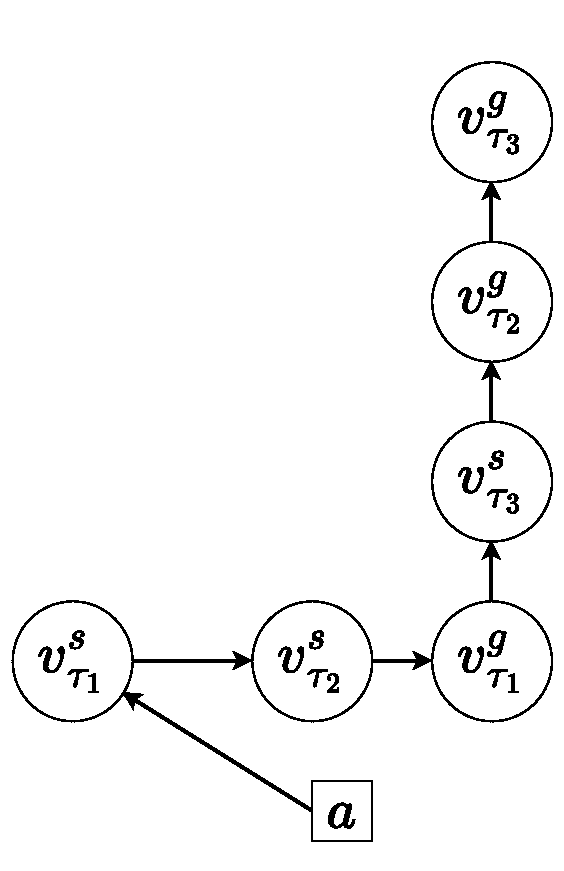
\includegraphics[width=0.3\linewidth]{Fig/A-TG.pdf}
    \caption{The schedule of agent $a$ to complete $\Gamma$}
    \label{fig:agent-taskgroup}
    \Description{The schedule of agent $a$ to complete $\Gamma$}
  \end{figure}
\end{example}

Therefore, to consider the location of agents,
we split the task group $\Gamma$ into multiple subgroups,
\begin{eqnarray}
  \label{eq:split}
  \Pi_{\Gamma} = \{ \forall \Gamma_i | \Gamma_i \subset \Gamma \}
\end{eqnarray}
where $\Pi_{\Gamma}$ is the set of subgroups of $\Gamma$.


Based on there,
we propose the Task Group Allocation Algorithm (TGA) to allocate task groups to agents.


\begin{algorithm}[htbp]
\caption{Task Group Allocation Algorithm}
\label{alg:TGA}
\begin{algorithmic}[1]
\Require Set of tasks $\Gamma$, set of agents $A$ %%input
\Ensure Set of schedule $\mathcal{S}_S$ of all agents %%output
\State $K$ = the max capacity of agents
\State $\Pi$ = K-Capacity Hierarchical Clustering Algorithm($\Gamma$, $K$)
\For {$\Gamma \in \Pi$}
    \State Get $\Pi_{\Gamma}$ by Equation~\ref{eq:split}
    \State ${\tilde{\Pi}}$ extends $\Pi_{\Gamma}$
\EndFor
\For {$a_i \in A$, $\Gamma_j \in {\tilde{\Pi}}$}
    \State Get detour cost $DCost(S_{\Gamma_{a_i}})$ by GSTG Algorithm
\EndFor
\While {${\tilde{\Pi}}$ is not empty}
    \State Select agent $a$ and task group $\Gamma$ with minimum detour cost
    \State Remove $\Gamma$ and $\forall \Gamma'| \Gamma'\cap \Gamma \neq \phi $
\EndWhile
\end{algorithmic}
\end{algorithm}

\textbf{Algorithm Detail:}
The pseduo-code of Task Group Allocation Algorithm is shown in Algorithm~\ref{alg:TGA},
where the input is a set of tasks $\Gamma$ and a set of agents $A$,
and the output is a set of schedule $\mathcal{S}_S$ of all agents.
First, we get the max capacity of agents $K$,
and call KCHC Algorithm to find a set of task groups $\Pi$ (lines 1-2).


\textbf{Analysis:}
% \balance

%%%%%%%%%%%%%%%%%%%%%%%%%%%%%%%%%%%%%%%%%%%%%%%%%%%%%%%%%%%%%%%%%%%%%%%%

%%% The acknowledgments section is defined using the "acks" environment
%%% (rather than an unnumbered section). The use of this environment 
%%% ensures the proper identification of the section in the article 
%%% metadata as well as the consistent spelling of the heading.
 
\begin{acks}
  This work is financially supported by Shenzhen Science and Technology Program 
  under Grant No.GXWD20220817124827001 and No.JCYJ20210324132406016.
\end{acks}

%%%%%%%%%%%%%%%%%%%%%%%%%%%%%%%%%%%%%%%%%%%%%%%%%%%%%%%%%%%%%%%%%%%%%%%%

%%% The next two lines define, first, the bibliography style to be 
%%% applied, and, second, the bibliography file to be used.

\bibliographystyle{ACM-Reference-Format} 
\bibliography{sample}

%%%%%%%%%%%%%%%%%%%%%%%%%%%%%%%%%%%%%%%%%%%%%%%%%%%%%%%%%%%%%%%%%%%%%%%%


\end{document}

%%%%%%%%%%%%%%%%%%%%%%%%%%%%%%%%%%%%%%%%%%%%%%%%%%%%%%%%%%%%%%%%%%%%%%%%

% \begin{algorithm}[ht]
% \caption{K-Capacity Hierarchical Clustering Algorithm}
% \label{alg:KCHC}
% \KwIn{Set of tasks $\Gamma$, the max capacity of agents $K$}
% \KwOut{Set of task groups ${\Pi}$}
% Initialize ${\Pi} = \emptyset$
% \For {$\tau_{i} \in \Gamma$}{
%     Treat $\tau_{i}$ as a task group $\Gamma_{i}$, and add $\Gamma_{i}$ into ${\Pi}$
%     Calculate the carpooling chance between $\tau_{i}$ and other tasks in $\Gamma$
% }
% \Return$\Pi$
% \end{algorithm}